\documentclass[14 pt]{article}
\usepackage{graphicx}
\usepackage{float}
\usepackage[english,russian]{babel}
\usepackage[a4paper, total={6in, 9in}]{geometry}
\usepackage{indentfirst}
\setlength{\parindent}{3em}


\title{Рассчётная работа}
\author{Дождиков Александр, гр. 421702}
\date{Декабрь 2024}

\begin{document}

\large
\maketitle
\newpage

\section{Введение}
\begin{введение}
В моём варианте рассчётной работы нужно было найти Минимальное и среднее расстояние между периферийными вершинами неориентированного графа.

Для того, чтобы реализовать данную задачу я использовал матрицу смежности и алгоритм Флойда-Уоршелла.
\end{введение}

\section{Алгоритм}
\begin{алгоритм}
Мой код реализует данный алгоритм:
\begin{itemize}
    \item В консоль выводится 6 вариантов опций. Пользователь может выбрать одно из пяти решений, либо завершить выполнение прораммы, выбрав 6 опцию:
    \begin{figure}[H]
    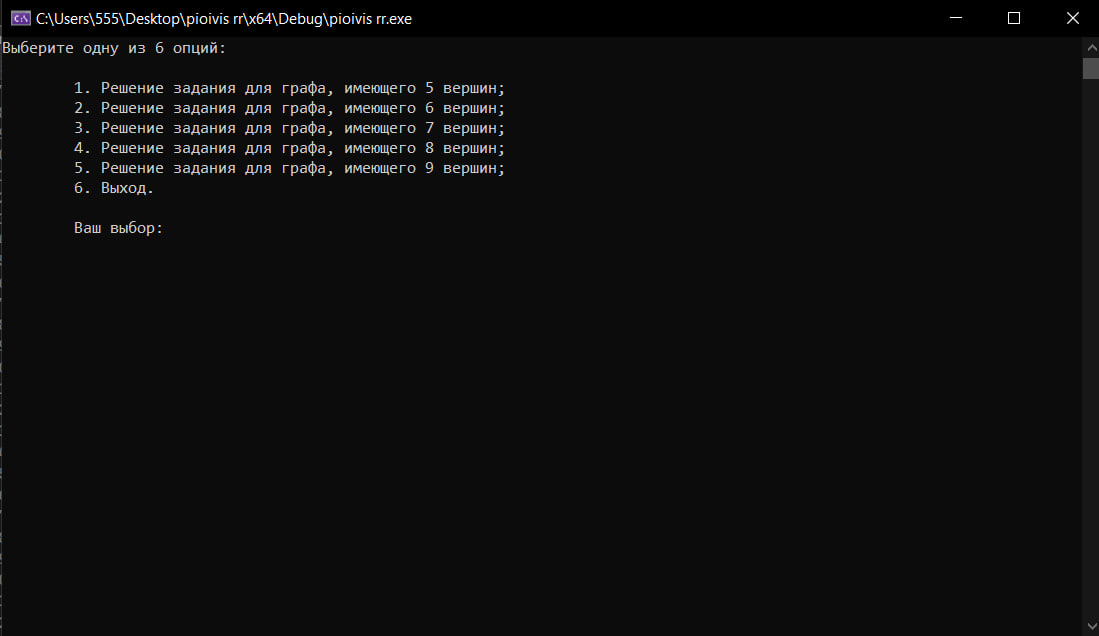
\includegraphics[width=10cm]{options.jpg}
    \centering
    \end{figure}
    \item Далее, при выборе одного из решений, через отдельную функцию абсолютно рандомно формируется матрица смежности для выбранного графа:
    \begin{figure}[H]
    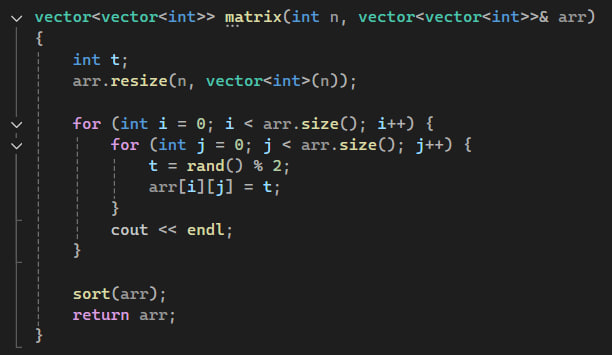
\includegraphics[width=7cm]{matrix.jpg}
    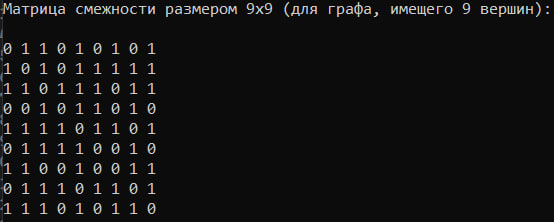
\includegraphics[width=7cm, height=4cm]{matrix9.jpg}
    \centering
    \end{figure}
    \newpage
    \item Далее, посредством алгоритма Флойда-Уоршелла, формируется матрица кратчайших путей, для нахождения минимального и среднего расстояния:
    \begin{figure}[H]
    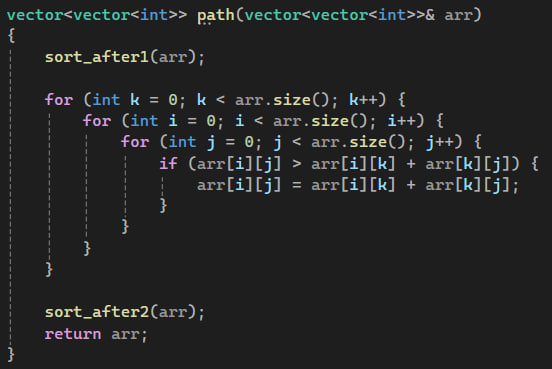
\includegraphics[width=10cm]{matrix1.jpg}
    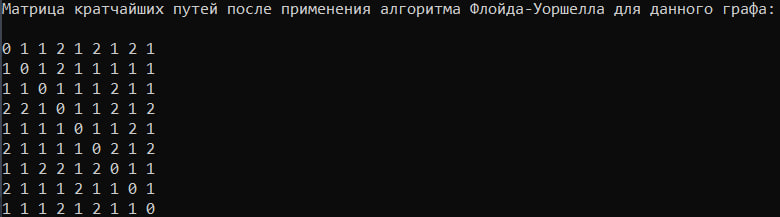
\includegraphics[width=10cm]{matrix99.jpg}
    \centering
    \end{figure}
    \item Далее, используя несколько сортировок, я находил минимальное и среднее расстояние между переферийными вершинами графа:
    \begin{figure}[H]
    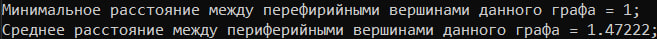
\includegraphics[width=10cm]{result.jpg}
    \centering
    \end{figure}
\end{itemize}
\end{алгоритм}
\section{Пример работы программы}
\begin{пример}
Пользователь выбирает первую опцию, которая выдаёт решение задания для графа, имеющего 5 вершин: 
\begin{figure}[H]
    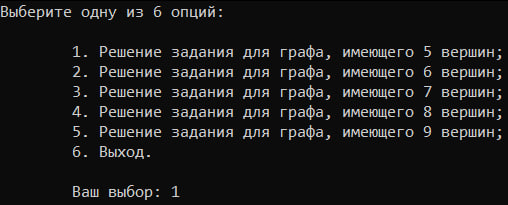
\includegraphics[width=10cm]{ex.jpg}
    \centering
    \end{figure}
\par
\newpage
Данный граф выглядит таким образом:
\begin{figure}[H]
    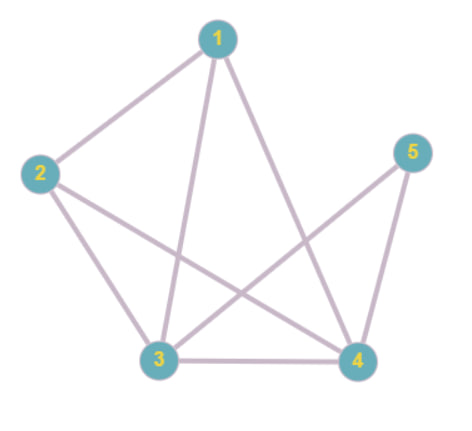
\includegraphics[width=10cm]{graph.jpg}
    \centering
\end{figure}
\par
После выбора первой опции, пользователь получает решение задания для данного графа:
\begin{figure}[H]
    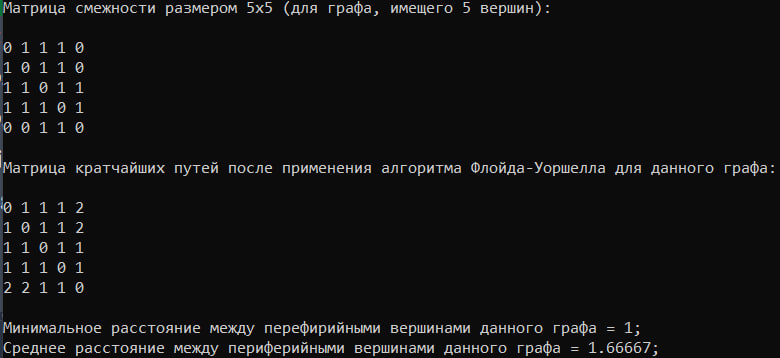
\includegraphics[width=13cm]{example.jpg}
    \centering
\end{figure}
\end{пример}
\section{Вывод}
\begin{вывод}
Во время выполнения рассчетной работы я ознакомился с понятием графов. Изучил, какие виды графов бывают (ориентированные/неориентированные, взвешенные/ невзвешенные). Ознакомился с таким способом представления графов в памяти компьютера, как список смежности. Также в ходе выполнения рассчетной работы реализовал алгоритм Флойда-Уоршелла на языке С++, проверил его работу.
\end{вывод}
\section{Источники}
\begin{источники}
1. Алгоритм Флойда-Уоршелла: https://ru.wikipedia.org/wiki
\par
2. Граф: https://ru.wikipedia.org/wiki
\par
3. Реализация алгоритмя Флойда-Уоршелла на практике: \par
https://rutube.ru/video/ffc617166c6d4cea7ec84699c263fd5b/
\end{источники}
\end{document}
